\documentclass[12pt,letterpaper]{scrreprt}

%----------------------------------------------------------------------
%				Required Packages
%----------------------------------------------------------------------
\usepackage{usecases}
\usepackage{enumitem}
\usepackage{graphicx}
%\usepackage{paralist}
%\usepackage{tabto}
\usepackage[top=2cm,bottom=3.5cm]{geometry}

%----------------------------------------------------------------------
%				Title Page
%----------------------------------------------------------------------
\title{CS383: Software Engineering}
\subtitle{HW2: Use Cases\\Spring 2014}
\author{Tao Zhang(zhan1872@vandals.uidaho.edu)\\
		John Goettsche(john.h.goettsche@gmail.com)\\
		Cameron Simon(simo2703@vandals.uidaho.edu)\\
		Gabriel Pearhill(pear9115@vandals.uidaho.edu)\\ 
		Wayne Fuhrman(fuhr0438@vandals.uidaho.edu)\\
		Joseph Higley(higley@vandals.uidaho.edu)} 
\date{}

%----------------------------------------------------------------------
%				Additional Settings
%----------------------------------------------------------------------
\setcounter{tocdepth}{3}
\setcounter{secnumdepth}{3}




%----------------------------------------------------------------------
%				Playtest Document Starts
%----------------------------------------------------------------------
\begin{document}

% Initializations
%\NumTabs{2} % This is for creating a two column use case scenario
\maketitle
\tableofcontents % Eventually uncomment this

\chapter{Description of Network}
\section{How does it look like?}
\paragraph{(Author: Tao Zhang)}
\paragraph{During the Main menu steps: }
\begin{itemize}
	\item Login/out: Each user should have an account. Once the user open the game, the user has to login with the account, otherwise register one (there will be a register button). What's more, we could add some features, like "Friend" System, which allows to invite friends to play.
	\item My suggestion is that we should not have Save and Resume, because that is kind of complex. A user want to end the game will be assumed that he want to surrander, instead of save a game. But if we want, here's the idea.
	\item Resume a game: Once the user claims to play a saved game, the server has to seek if all the players for this game are online. Then send a message to all the users that invite them to play the game. If all the users accept, the server will read the data and reset everything from last time on the screen.
	\item Save a game: If a user claimed to save a game, and all other users agree, the game will be saved and end. Server will save the data
	\item New Match: If a user claimed to play a new senario, the server can search the users who also want to play this senario and randomly choose users to make a new game.
\end{itemize}

\paragraph{For each game turn:}
\begin{itemize}
	\item Roll dices: randomly compute two numbers in order.
	\item Random events: Compute the random events and inform that. Then update all the information on each user's screen.
	\item Player order: Compute the random order, then server controls the order and let each user to take their turns.
	\item Random movement: server will compute randomly movements and update that on user's screen
	\item Diplomacy: 
	\item Mana Regeneration: Server will compute and plus all mana regenerated for each character, update on user's screen
\end{itemize}

\paragraph{Then during the player's turn, the networked multi-player system record the finial decision from one user, then transfer and display the information on other users's screen.}
\begin{itemize}
	\item For example, in the movement, each time the phasing player informs a character movement, the server will read the data and transfer to other user's local directory, then update the screen.
	\item Special cases: after phasing player claimed "end of spell segment". Phasing player will lost the right to operate, server will transfer the right to other users. Server then wait all other non-phasing players' claim of "end of counterspell segment". Server operate all the counterspells on all users screen and return the right to phasing player.
\end{itemize}

\paragraph{Finally, the most important thing I considered is that we have to create temperaty files in all user's local directories. These files are used to record all operations among the players and server, which:}
\begin{itemize}
	\item Record local user's operations immediately 
	\item Server read the file and transfer to all other user's local temp files
	\item Local PC reads the updated temp file and operate the update on user's screen
\end{itemize}


\chapter{Use Case Diagrams}

\section{General (Tao)}
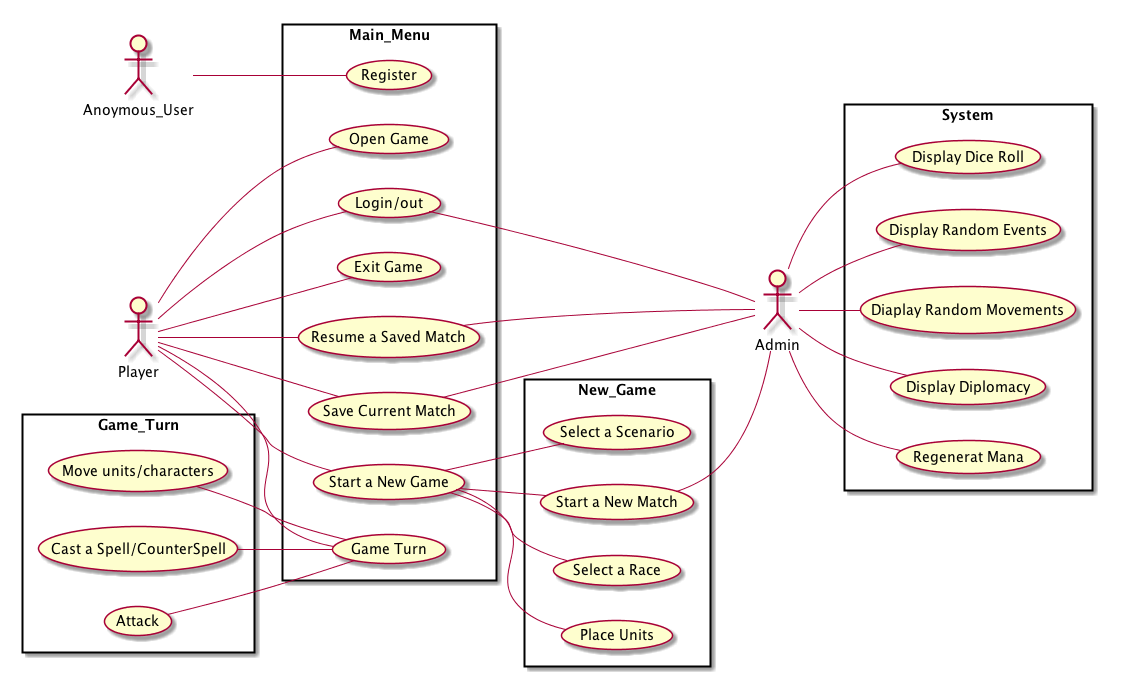
\includegraphics[scale=0.4]{Tao-usecase-diagrams.png} 
\section{Main Menu (Wayne)}
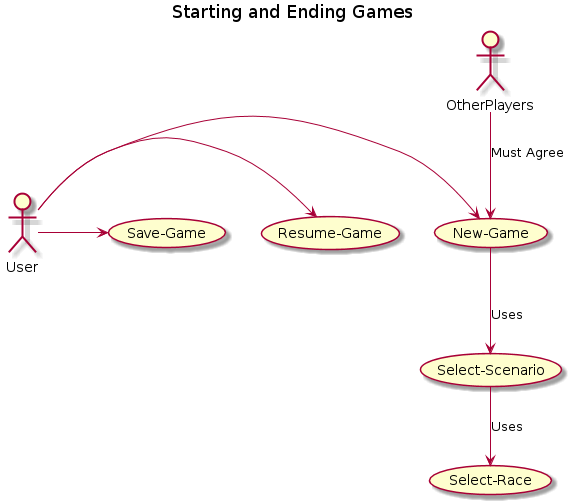
\includegraphics[scale=0.6]{menuSelection.png}
\section{Random Events (John)}
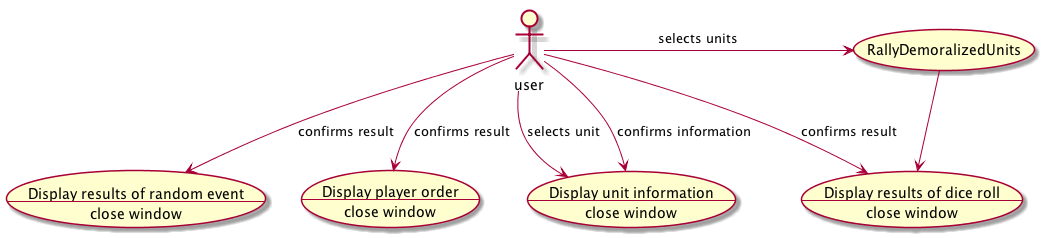
\includegraphics[scale=0.4]{usecasesJohn.png}
\section{Movement (Gabe)}
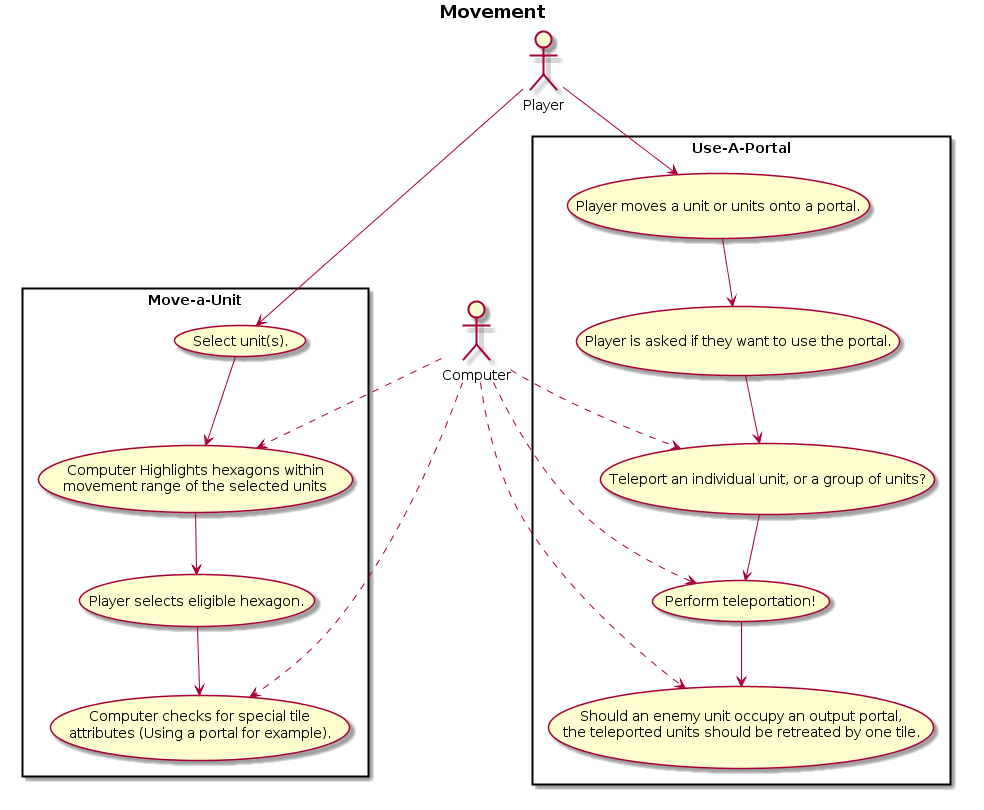
\includegraphics[scale=0.5]{MovementUseCaseDiagrams.png}
\newpage
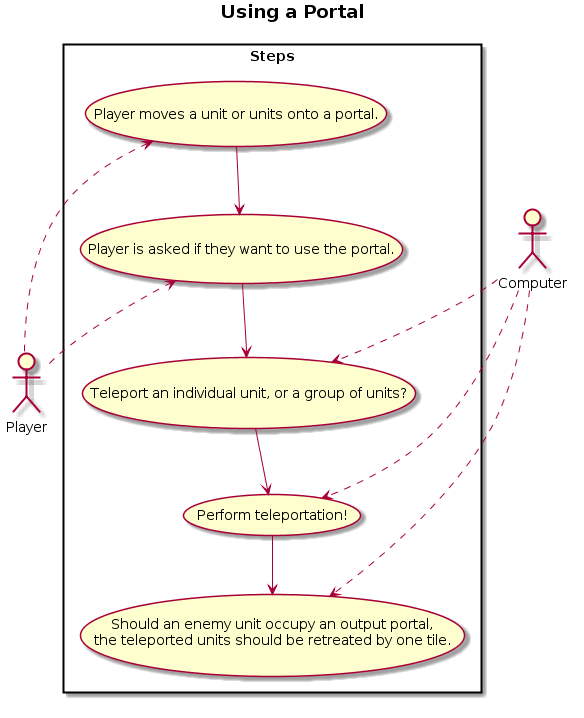
\includegraphics[scale=0.6]{PortalUseCaseDiagram.png}
\section{Magic (Tao)}
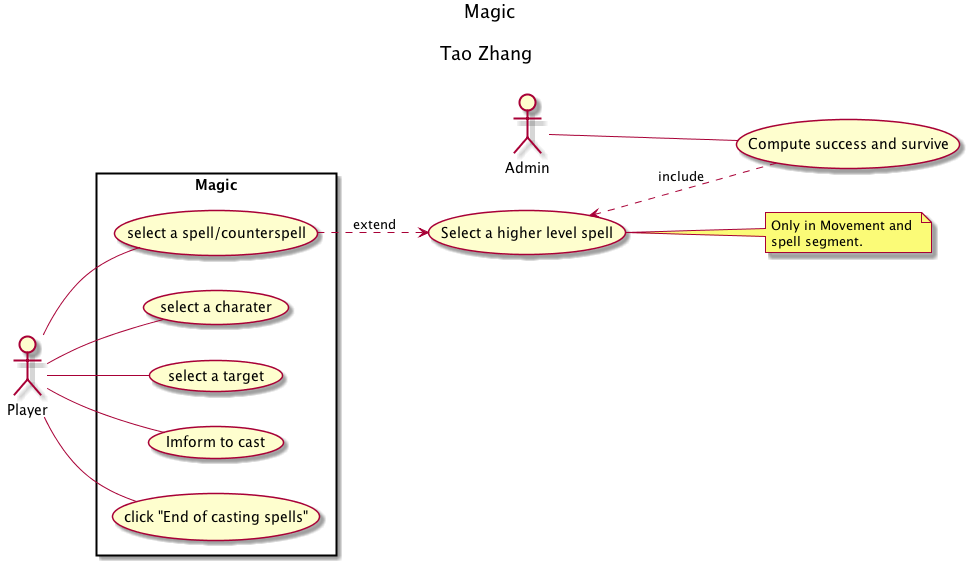
\includegraphics[scale=0.4]{MagicDiagram.png}
\section{Diplomacy (Cameron)}
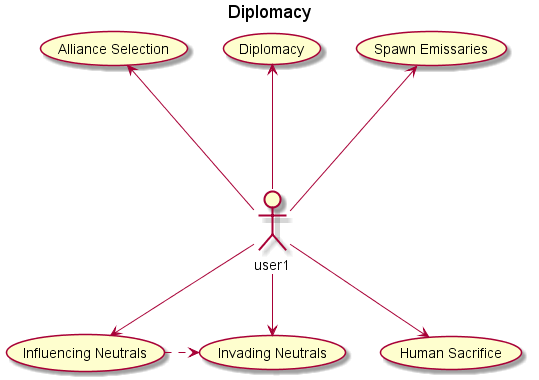
\includegraphics[scale=0.6]{DiplomacyUseCaseDiagram.png}


%----------------------------------------------------------------------
%				Use Case Document Starts
%----------------------------------------------------------------------
\chapter{Use Cases Descriptions}

%----------------------------------------------------------------------
%					Random Events: John Goettsche
%----------------------------------------------------------------------
\section{Random Events}
\paragraph{(Author: John Goettsche)}
	\subsection{Display Die Roll}
		\begin{usecase}
			\addtitle{Random Events}{Dispay Die Roll}
			\addfield{Summary}{Displays the result of a die roll}
			\additemizedfield{Actors}{
				\item Players		
			}
			\additemizedfield{Preconditions}{
				\item A die roll is required for a user command
			}
			\addscenario{Primary Sequence}{
				\item user selects a command that requires a die roll
				\item Computer selects a random number from 1 to 6
				\item Computer displays message box with selected value
				\item User clicks OK button
				\item Computer closes message box
			}
			\additemizedfield{Alternatives}{
				\item Computer requires more than one die roll, then the process is performed the number of times it is requested
			}
			\additemizedfield{Postconditions}{
				\item a random number from 1 to 6
			}
		\end{usecase}	
		
	\subsection{Display Player Order}
		\begin{usecase}
			\addtitle{Random Events}{Display Player Order}
			\addfield{Summary}{display the order of play}
			\additemizedfield{Actors}{
				\item Players	
			}
			\additemizedfield{Preconditions}{
				\item is currently the Player-Order Determination Inter-Phase
			}
			\addscenario{Primary Sequence}{
				\item Computer determines the order of play
				\item Computer displays a dialog box with the order of play
				\item User clicks the OK button
				\item Computer closes dialog box
			}
			\additemizedfield{Postconditions}{
				\item a message box informing the user of the order of play
			}
		\end{usecase}			
		
	\subsection{Display Random Events}
		\begin{usecase}
			\addtitle{Random Events}{Display Random Events}
			\addfield{Summary}{displays a dialog box describing a random event}
			\additemizedfield{Actors}{
				\item Players
			}
			\additemizedfield{Preconditions}{
				\item is currently the Random Event Determination Inter-Phase
			}
			\addscenario{Primary Sequence}{
				\item Computer selects a random event
				\item Computer displays a dialog box describing the random event.
				\item User selects the OK button
				\item Computer closes dialog box
			}
			\additemizedfield{Postconditions}{
				\item a dialog box describing a random event
			}
		\end{usecase}	

		
	\subsection{Display Random Movement}
		\begin{usecase}
			\addtitle{Random Events}{Display Random Movement}
			\addfield{Summary}{move all the vortices, uncontrolled killer penguins, or other randomly-moving units or characters which are required to move in this phase}
			\addscenario{Primary Sequence}{
				\item Computer centers on the view on a unit to be moved
				\item Computer moves the unit
			}
			\additemizedfield{Postconditions}{
				\item each move is displayed on the screen
			}
		\end{usecase}		
	
	\subsection{Rally Demoralized Units}
		\begin{usecase}
			\addtitle{Random Events}{Rally Demoralized Units}
			\addfield{Goals}{User rallies demoralized units.}
			\additemizedfield{Actors}{
				\item Players
			}
			\additemizedfield{Preconditions}{
				\item is currently a players Combat Phase
			}
			\addfield{Summary}{User attempts to rally units}
			\addscenario{Primary Sequence}{
				\item user selects a unit to rally (see Unit Selection)
				\item Computer determines if the rally was 
				\item Computer displays the die roll (see Display Die Roll)
				\item Computer displays the unit in its new status (demoralized or not 
			}
			\additemizedfield{Postconditions}{
				\item a potential change in status for demoralized unit
			}
		\end{usecase}		
		
	\subsection{Display Unit}
		\begin{usecase}
			\addtitle{Random Events}{Display Unit}
			\addfield{Goals}{Display unit information}
			\additemizedfield{Actors}{
				\item Players
			}
			\additemizedfield{Preconditions}{
				\item User turn
			}
			\addfield{Summary}{display a message box showing information about a selected unit}
			\addscenario{Primary Sequence}{
				\item User selects a unit
				\item Computer displays a message box containing all the relavant information on the unit
				\item User selects the OK button
				\item Computer closes the message box
			}
			\additemizedfield{Postconditions}{
				\item a dialog box displaying the unit information
			}
		\end{usecase}				
		
		

%========================================================
%	Selection Section - Gabe Pearhill
%========================================================                         
\section{Selection}
\paragraph{(Author: Gabe Pearhill)}
            \subsection{Unit Selection}
                \begin{usecase}
                  \addtitle{Select Unit(s)}{Select one or more units}
                  \addfield{Summary}{Player clicks a unit on the game board.}
                  \additemizedfield{Actors}{
                    \item Player
                  }
                  \additemizedfield{Preconditions}{
                    \item Phase requiring unit selection.
                  }
                  \addscenario{Steps}{
                    \item Once a phase requiring unit selection begins, the computer highlights all available units. 
                    \item The user clicks one or more units.
                    \item Computer saves the selection state.
                  }
                  \end{usecase}
                
                 
            \subsection{Hexagon Selection}
                \begin{usecase}
                  \addtitle{Select Hexagon}{Record the players hexagon selection.}
                  \addfield{Summary}{The basic action of selecting a hexagon, be it for magic, movement, or attacking.}
                  \additemizedfield{Actors}{
                        \item Player
                  }
                  \addscenario{Steps}{
                                    \item Player clicks on a hex.
                                    \item Computer records the hex selection.
                  }
                \end{usecase}

%========================================
%	Movement Section - Gabe Pearhill
%========================================
\section{Movement}
\paragraph{(Author: Gabe Pearhill)}
            \subsection{Move a Unit}
                \begin{usecase}
                  \addtitle{Move Unit(s)}{Move unit(s) across the map!}
                  \addfield{Summary}{During the movement phase the player selects and moves units.}
                  \additemizedfield{Actors}{
                    \item Player
                  }
                  \additemizedfield{Preconditions}{
                    \item Movement Phase
                  }
                  \addscenario{Steps}{
                    \item Select unit(s). (See Unit Selection)
                    \item Computer highlights hexagons within range of the selected units.
                    \item Player selects an eligible hexagon.
                    \item Computer checks if tile has special attributes (a portal for example) and takes action appropriately.
                    \item Handle items relating to zone of control.
                  }
                  \end{usecase}
                
                 
            \subsection{Using a Portal}
                \begin{usecase}
                  \addtitle{Teleportation}{Give the player the choice to use a portal hexagon.}
                  \addfield{Summary}{If a unit moves on top of a portal, and the player chooses to use it, the computer must move the selected units to another portal location on the map.}
                  \additemizedfield{Actors}{
                        \item Player
                  }
                  \addscenario{Steps}{
                                    \item Player moves on top of a portal hexagon.
                                    \item Player is provided a dialog giving them the option to use the portal.
                                    \item If the player chooses to use the portal the player must then choose to teleport his units individually or as a group.
                                    \item Perform appropriate teleportation.
                                    \item Should an enemy unit occupy an output portal, the teleported  units should be retreated by one tile.
                  }
                \end{usecase}
                
%==================================================
%				Magic: Tao Zhang
%==================================================
\section{Magic}
\paragraph{(Author: Tao Zhang)}
            \subsection{Cast a Spell}
                \begin{usecase}
                  \addtitle{Magic I}{Cast a Spell}
                  \additemizedfield{Actors}{
                    \item Phasing player
                  }
                  \addfield{Goal}{Phasing player cast spells}
                  \additemizedfield{Preconditions}{
                    \item Phasing player is in one of the following phase
                    	\begin{enumerate}
                    		\item Movement
                    		\item Spell Segment
                    		\item Combat
                    	\end{enumerate}
                  }
                  \addfield{Summary}{Phasing player gonna cast enough spells he want during his turn}
                  \additemizedfield{Related Usecases}{
                  	\item Movement
                  	\item Combat                  
                  }
                  \addscenario{Steps}{
                  	\item Phasing Player select a character with PL
					\item Phasing player select an available spell
					\item player selects a target for the spell
					\item Player imform to cast this spell
					\item repeat to cast enough spells
                  }
                  \additemizedfield{Alternative}{
					\item Only in Movement and spell segment:
						\begin{enumerate}
							\item Phasing player can choose a higher level spell with warning red background.
							\item Computer will computes the result if successfully cast the spell and whether the charater survive or not
						\end{enumerate}	
					\item Player click on the buttom "End of casting spells" which the bottom will always be displayed on side of the screen					               
                  }
                \end{usecase}
                
                \subsection{Cast a CounterSpell}
                \begin{usecase}
                  \addtitle{Magic II}{Cast a CounterSpell}
                  \additemizedfield{Actors}{
                  	\item Non-phasing Player
                  }
                  \addfield{Goal}{Non-phasing players cast counterspells}
                  \additemizedfield{Preconditions}{
                  	\item End of phasing player's spell segment
                  }
                  \addfield{Summary}{All non-phasing player will do this at the same time, and once all of them have clicked the "end of counterspell" button. The server will then turn to let phasing player control}
                  \addscenario{Steps}{
                  	\item Non-phasing player select a charater with PL
					\item Select an available counterspell
					\item Select a target to cast this spell
					\item Repeat to select enough counterspells
                  }
                  \additemizedfield{Alternative}{
                  	\item Non-phasing player click the button "End of casting counterspells". 
                  }
                  
                \end{usecase}
                
%=======================================================
%				Diplomacy: Cameron Simon
%=======================================================
\section{Diplomacy}
\paragraph{(Author: Cameron Simon)}
            \subsection{Influencing Neutrals}
                \begin{usecase}
                  \additemizedfield{Actors}{
                    \item User
                    \item Computer
                  }
                  \addfield{Goals: }{Influence Neutrals}
                  \additemizedfield{Preconditions}{
                    \item Neutral's Diplomacy marker must be within one hex of a lettered hex(a players hex) on the Diplomacy track. 
                  }
                  \addfield{Summary}{When a neutral is influenced by a player that player can move freely through that neutrals territory.}                  
                  \addscenario{Primary Sequence:}{
                        \item Computer recognizes neutral is being influenced by player.
                        \item Player prompted to see if they want to move through neutral territory.
                        \item Player moves through the neutrals territory as they wish.
                        \item If neutrals diplomacy marker is moved should prompt player to move out of neutral territory unless they want to enter "Invading Neutral" state.
                  }
                  \addfield{Produces: }{Diplomacy map with new neutral locations is displayed.}                  
              
                 \end{usecase}
                 
            \subsection{Invading Neutrals}
                \begin{usecase}
                  \additemizedfield{Actors}{
                    \item User
                    \item Computer
                  }
                  \addfield{Goals: }{Invade Neutrals}
                  \additemizedfield{Preconditions}{
                    \item User places his/her Army units, Monsters, or Vortices inside territories owned by a Neutral. 
                  }
                  \addfield{Summary}{Decide who neutrals in question are going to make alliances with.}                  
                  \addscenario{Primary Sequence:}{
                        \item Computer checks position of Neutral's Diplomacy marker on Diplomacy Track.
                        \item If marker is closest to a lettered hex, Computer places Neutral on side it was leaning toward.
                        \item If marker equidistant from two or more opposing, non-invading players, computer displays die roll and players roll (highest wins control). Computer places neutral in winning players hex.
                        \item If marker equidistant from invading player's hex and one or more other player's hex, it will immediately ally with some non-invading players as in step 3. Computer places neutral in winning players hex.
                        \item If marker closest to invading Player's hex it is immediately placed in Neutral central hex by computer.
                  }
                  \addfield{Produces: }{Diplomacy map with new neutral locations is displayed.}                  
              
                 \end{usecase}
                 
            \subsection{Human Sacrifice}
                \begin{usecase}
                  \additemizedfield{Actors}{
                    \item User
                    \item Computer
                  }
                  \addfield{Goals: }{Try to gain Influence over Neutrals}
                  \additemizedfield{Preconditions}{
                    \item Player moves a unit or Character adjacent to a unit or character controlled by the Neutral to whom he wishes to sacrifice. 
                  }
                  \addfield{Summary}{Neutral's Diplomacy marker is moved one hex by the sacrificing Player. }                  
                  \addscenario{Primary Sequence:}{
                        \item Player chooses option of human sacrifice.
                        \item During the Alliance Determination Phase, the unit or Character is removed from play by the computer.
                        \item Computer moves Neutral's diplomacy marker one hex.
                        \item Player may sacrifice as many units/characters as they wish but computer will NOT move diplomacy marker any more for that game turn.
                  }
                  \addfield{Produces: }{Diplomacy map with new diplomacy locations.}                  
              
                 \end{usecase}
                 
            \subsection{Spawn Emissaries}
                \begin{usecase}
                  \additemizedfield{Actors}{
                    \item User
                    \item Computer
                  }
                  \addfield{Goals: }{Creation of emissarries.}
                  \additemizedfield{Preconditions}{
                    \item Character must have diplomatic rating greater than zero.
                  }
                  \addfield{Summary}{Up to two emissaries created for character that exist only for one purpose. }                  
                  \addscenario{Primary Sequence:}{
                        \item Computer recognizes game is in Friendly Movement Phase.
                        \item Computer prompts user to see if they want to create emissaries.
                        \item User responds yes or no.
                        \item User selects how many they want to create (1 or 2).
                  }
                  \addfield{Produces: }{Specified number of emissaries on game board. (Do we need rules for emissary movement and  deletion in this use case?)}                  
              
                 \end{usecase}
                 
                \subsection{Diplomacy}
                \begin{usecase}
                  \addtitle{Author: } {Cameron Simon}
                  \additemizedfield{Actors}{
                    \item User
                    \item Computer
                  }
                  \addfield{Goals: }{Establish new diplomacy lines on table.}
                  \additemizedfield{Preconditions}{
                    \item Game must be in Diplomacy Inter-Phase state and a player must have a Character of Emissary in the Capital hex of a Neutral Power. 
                  }
                  \addfield{Summary}{Establish new diplomacy lines based on game specifications.}                  
                  \addscenario{Primary Sequence:}{
                        \item Computer cross references the race of the player's character or emissary and the race of the neutral power on the table to yield a single number (negative or positive).
                        \item Player rolls two dice and has that number added to the number found in step 1.
                        \item Computer references the Diplomacy Results table with number found above (result will be positive, negative, or an 'x').
                        \item Based on output from step 3 and the rule specification for those outputs, the computer places the pieces in their new locations on the diplomacy track.
                  }
                  \addfield{Produces: }{Display updated map with new marker location on diplomacy map.}                  
              
                 \end{usecase}
                 
            \subsection{Alliance Selection}
                \begin{usecase}
                  \additemizedfield{Actors}{
                    \item User
                    \item Computer
                  }
                  \addfield{Goals: }{Form alliances with other players.}
                  \additemizedfield{Preconditions}{
                    \item Game must be in Player-Order Determination Inter-Phase. 
                  }
                  \addfield{Summary}{Players choose who they want to be allied with for the current game turn.}                  
                  \addscenario{Primary Sequence:}{
                        \item Each player is prompted to see if they want to form alliances.
                        \item If player says yes, then they select the player they want to ally with.
                        \item Computer checks to see if players selected each other to be allies. (Ex: If player A selects to ally with player B, Player B must also select to ally with player A to form the alliance)
                  }
                  \addfield{Produces: }{Displays current player alliances.}                  
              
                 \end{usecase}             


                 
\end{document}
